\documentclass{article}

\usepackage{graphicx}
\usepackage{onecolceurws}
\usepackage{amssymb}
\usepackage{amsfonts}
%\usepackage{amsmath}
\usepackage{url}
\usepackage{listings}
\usepackage{authblk}

\title{Deduction as a Service}

\author{Mohamed Bassem Hassona\\German University in Cairo\\
{\small \tt mohamed.hassona@student.guc.edu.eg}
\and
Stephan Schulz\\DHBW Stuttgart\\{\small \tt schulz@eprover.org}}

\institution{}

%\author{Mohamed Bassem Hassona}
%
%\affil{German University in Cairo \authorcr{}{\small \tt mohamed.hassona@student.guc.edu.eg}}
%\author{Stephan Schulz}
%\affil{DHBW Stuttgart\authorcr{\small \tt schulz@eprover.org}}

\date{}

\newcommand{\mw}[1]{\ensuremath{\mathit{#1}}}
\newcommand{\nat}{\ensuremath{\mathbb N}}
\newcommand{\integer}{\ensuremath{\mathbb Z}}
\newcommand{\rat}{\ensuremath{\mathbb Q}}
\newcommand{\real}{\ensuremath{\mathbb R}}
\newcommand{\eqn}[2]{\ensuremath{#1\!\simeq\!#2}}
\newcommand{\neqn}[2]{\ensuremath{#1\!\not\simeq\!#2}}
\newcommand{\ueqn}[2]{\ensuremath{#1\dot{\simeq}#2}}

\newcommand{\terms}{\ensuremath{\mathit{Term(F,V)}}}
\newcommand{\tops}{\mathop{\mathrm{top}}\nolimits}
\newcommand{\pos}{\mathop{\mathrm{pos}}\nolimits}
\newcommand{\gfpf}{\mathop{\mathrm{gfpf}}\nolimits}
\newcommand{\fpf}{\mathop{\mathrm{fpf}}\nolimits}
\newcommand{\fp}{\mathop{\mathrm{fp}}\nolimits}
\newcommand{\text}[1] {\mbox{#1}}

\renewcommand{\textfraction}{.05}
\renewcommand{\topfraction}{.95}
\renewcommand{\bottomfraction}{.95}


\lstset{frame=tb,
  aboveskip=3mm,
  belowskip=3mm,
  showstringspaces=false,
  columns=flexible,
  basicstyle={\small\ttfamily},
  breaklines=true,
  breakatwhitespace=true,
  tabsize=2
}

%\pagestyle{empty}
%\bibliographystyle{alpha}
%\bibliographystyle{splncs03}

\begin{document}
\bibliographystyle{plain}

\maketitle

\begin{abstract}
  We describe a system offering deduction (over a fixed but flexible
  background theory) as a service, provided to a client via a network
  connection. The deduction server maintains the (potentially) large
  background knowledge base in a form that makes processing of
  individual conjectures and queries easy and avoids most of the
  overhead of reading and analyzing large background theories for each
  individual job. The client connects to the server, can update the
  background theory by adding and removing client-side or server-side
  axiom sets, and ask the server to solve proof problems on its
  behalf.

  This offers several benefits: Preprocessing costs can be amortized
  over multiple proof attempts. The user can be isolated from the
  complexities of a locally installed ATP system (and indeed locally
  maintained knowledge bases). Finally, the deduction server can
  easily offer true strategy parallelism even with sequential back-end
  theorem provers.

  This paper describes the architecture, the communication protocol,
  and the implementation of a deduction server based on E. First
  experimental results demonstrate the feasibility of the technology
  and the performance benefits possible with this approach.
\end{abstract}

\section{Introduction}
\label{sec:intro}

Classical automated theorem proving has long been concerned with
solving individual problems, one at a time. Moreover, problems have
often been hand-optimized, either to solve a particular mathematical
question, or to analyze and demonstrate the performance of different
theorem proving strategies (see e.g.~\cite{McCune:Wos-1997}). One of
the best-knows examples is McCune's formalization and ultimate proof of
the Robbins problem~\cite{McCune:JAR-1997}.

However, in recent years, theorem provers have been used in a very
different setting. Users have developed large theories, either by
large-scale manual coding of knowledge as in Cyc~\cite{RRG:CO-2005} or
SUMO~\cite{PNL:AAAIWS-2002}, by organized efforts to formalize
significant parts of mathematics (e.g.~MIZAR~\cite{TB:IJCAI-1985}, or
more recently Flyspeck~\cite{HHMNOZ:Kepler-2011}), or from the
verification of large systems like the sel4
micro-kernel~\cite{KE:SOSP-2009}. These theories are typically
developed in either an interactive theorem prover, or in authoring
environment like Sigma-KEE~\cite{PS:IJCAR-2014}. Automated theorem
provers can be used to dispose a significant number of sub-problems
that can be translated into first-order logic. Examples are MizAR for
MIZAR and the various ``Hammers'' for
Isabelle~\cite{MP:JAL-2007,MP:JAR-2009,BN:IJCAR-2010} and HOL
Light/HOL~ 4~\cite{KU:JAR-2014,GK:CPP-2015}. Communication between
interactive and local automatic systems is usually via an ad-hoc
protocol. As a fallback, some interactive prover also use the TPTP
World web service~\cite{Sutcliffe:LPAR-2010} to invoke remotely
installed ATP systems.

In these newer use cases, the theorem prover proves and reproves many
different theorems over a large and mostly static background
theory. Typically, the background theory has thousands to millions of
axioms, only a small fraction of which is used for any given
proof. Premise selection
techniques~\cite{HV:CADE-2011,KLTUH:CADE-2012,GK:CPP-2015} enable
provers to handle such large problems. However, for large problems,
parsing and preprocessing takes significant amounts of
time.\footnote{As an example, E takes around 54 seconds (on a system
  with a 4 GHz Intel i7 and a fast SSD) just to parse the TPTP problem
  \texttt{CSR073+6.p}, a first-order problem based on OpenCyc with
  nearly 3.5 million axioms and taking up 480~MB. Indexing for SInE
  axiom selection takes a further 2 seconds, while more than half of
  successful proof attempts need less than 1 second.}

In this paper, we suggest a different paradigm. Deduction, over a
fixed but flexible base theory, is offered as a network service. The
deduction server maintains a knowledge base of several pre-loaded
background axiomatization. The user can connect to the server, select
specific parts of the knowledge base, add additional assumptions, and
then request a proof from the server. The server combines the
pre-loaded and pre-indexed background theory with the new formulas
provided by the user, runs several premise selection strategies to
generate ATP problems, and runs several ATP instances with different
heuristics to try to solve the problem. If one of the server processes
finds a proof, it is handed back to the client.

This approach has a number of advantages. First, the cost of loading
and pre-processing the large background theory is amortized over many
different proof problems. Proofs to individual problems are often
found fast and with low latency. The user can prepare and issue
queries from a local desktop, while the deduction server can be shared
by several users and run on powerful server hardware. Indeed, the user
does not even need to know how to install or invoke ATP systems, since
the server can be centrally installed and maintained. 

We have developed a suitable communication protocol and implemented a
deduction server based on the theorem prover
E\cite{Schulz:AICOM-2002,Schulz:LPAR-2013} and its libraries of data
types and algorithms for deduction. First results show that the
approach is feasible, and that the overhead for processing large
problems can be significantly reduced. In the following sections we
describe the design, architecture, and implementation of the deduction
server, and provide data about a first experimental evaluation.

The system is available
at~\url{http://www.eprover.eu/E-eu/DedServer.html}, and will become
part of future distributions of E.


\section{Client-Server Architecture}

\subsection{Deduction Server}

The deduction server is the central component for offering
\emph{Deduction as a Service}. It maintains the current state of the
knowledge base, accepts connections from clients, reads and processes
their requests, runs deduction jobs on behalf of the clients, and
transmits the results back to the client. The main architectural
components of the server are the knowledge base, the TCP interface,
the axiom filter, and the execution module.

At start-up, the server starts listening on a user-specified port for
incoming TCP connections. Whenever a client tries to connect to the
server on that port, a process is forked from the main process to
serve the client. The server can thus handle several different
connections at the same time, and each client is completely isolated
from other clients connected to the server.

The client interacts with the server using the protocol specified in
section~\ref{sec:prot}. The server implements a typical
read-execute-print loop, accepting commands from the client, executing
them, and sending the results back to the client. The client can
upload axiom sets, remove them, and query the server for proofs and
answers (i.e.\ instantiations of variables that make an existentially
quantified query formula true~\cite{SSSU:TPTP-ANS}).

Whenever the client uploads a set of axioms, the server parses the
axioms, adds them to various indexes useful for axiom
selection/pruning methods, and adds them to the in-memory knowledge
base. However, these uploaded axiom sets will not automatically be
used by each proof attempt, but only when the client has also
activated (or \emph{staged}) the particular set in the current
session. Thus, the server maintains a pre-indexed, ready-to-use
library of axiom sets. In addition to axiom sets uploaded by the
client, the server can also offer access to axiom sets stored in a
server-side library on disk. Axioms loaded by the server on start-up
are available to all users, while axiom sets added by a user during a
session are currently only available in that session.

After the client chooses some axiom sets to be used in the proof
search, it can start querying the server. The query consists of
optional query-specific axioms and a conjecture. These additional
formulas are discarded immediately after the query has been
processed. The server adds the new axiom set to the currently staged
part of the knowledge base and hands the problem to the axiom
filter. The axiom filter module applies one or multiple different
relevancy pruning strategies to the extended knowledge base. Each of
the pruning strategies produces one much smaller proof problem. The
pruned problems are passed to the execution module, which starts
several instances of E in parallel and monitors their success or
failure. Whenever one of the running E instances finds a proof for the
conjecture, the other instances are stopped and the proof is returned
back to the user. Currently, all instanced of E use its conventional
\emph{automatic mode}, and rely on the different pruning strategies to
provide diversity for the proof attempt.

The rough architecture of the deduction server is shown in
Figure~\ref{deduction_server_figure}.

\begin{figure}[t]
  \centering
  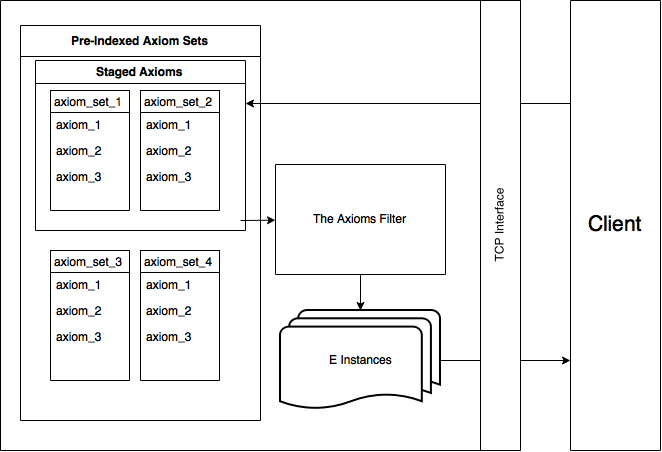
\includegraphics[width=0.9\textwidth]{imgs/TheDeductionServer.png}
  \caption{The Deduction Server Architecture\label{deduction_server_figure}}
\end{figure}

The deduction server is written in C and integrated with the E
distribution. It uses the E libraries and data types to parse and
represent logical formulas, to maintain and process first order
knowledge bases, and to perform axiom selection.


\subsection{User client}

The E distribution includes a small Python client called
``enetcat.py'', which can be used to interact with the server. The
client is intended as a reference implementation, to demonstrate the
interactions with the server and enable other developers to use it as
a model for interfacing the server with other systems.

The client requires the address and the port of the deduction server
as arguments. It opens a TCP connection to the server and then reads
the user's commands from ``stdin'', communicates them to the server,
and prints the output back to ``stdout''.

In addition to encoding the plain text commands into the distinct
length-delimited TCP messages expected by the server, the client
offers two convenience features. First, it offers command line
editing. Secondly, it locally expands TPTP style \texttt{include}
commands for formula sets to be uploaded to the server. This makes
uploading of even large axioms sets plausible and convenient.

The current client is tailored towards command-line users. However,
the protocol is simple enough to be implemented in a few lines of code
in nearly any modern programming language, making other clients, in
particular a web-based client, easily possible.

%Having different implementations of the client in different
%programming languages makes it easier for complex systems to integrate
%with automated theorem provers and use them as a service. By just
%including the library, those systems don't need to have the ATP
%installed on their machines and don't need to care about the memory or
%the computation power needed for the proofs as proving conjectures is
%the server's responsibility.

\subsection{Communication Protocol}
\label{sec:prot}

As mentioned before, the communication between the server and the
client is done over TCP to ensure reliability. TCP messages between
the server and the client are encoded in a way to ease the
communication between them. Each TCP messages starts with 4 bytes
containing the length of the messages, including those 4 bytes,
followed by the actual message. The commands themselves are plain,
human-readable ASCII text.

We describe the protocol for communication between the server and the
client using a running example. We assume that the connection has
already been established and all messages are encoded as described in
the previous paragraph.

The first section of the session uploads two small axiom sets to the
server.  

\lstinputlisting[numbers=left]{codes/protocolexample1.txt} Each of the
``ADD \ldots GO'' blocks upload one named set of axioms to the
system. Axioms uploaded are parsed and stored in the memory of the
server, but are not automatically included in future proof
attempts. The server responds with the success status of each
command's execution.

\lstinputlisting[numbers=left]{codes/protocolexample2.txt} To select
axiom sets for future proof attempts, we use the ``STAGE'' command. It
marks the named axiom set as active for later proof attempts. The
``LIST'' command provides the status of all axiom sets currently known
to the server. Possible states are \emph{Staged}, \emph{Unstaged} (but
in memory and pre-indexed for axiom selection), and \emph{On Disk},
i.e.\ known to the server, but not loaded or indexed. Server-side
axiom sets can be loaded into the server's memory using the ``LOAD''
command.

\lstinputlisting[numbers=left]{codes/protocolexample3.txt} After
staging the needed axioms, we can start running a job with ``RUN
\ldots GO'' block. Formulas introduced in the RUN command block are
used only temporally for this particular job, and are discarded after
its termination. These formulas typically contain the conjecture, but
can also include additional axioms and assumptions. If the server
succeeds in proving the conjecture, it provides back the logical
status of the query, and can also include a proof object.

\lstinputlisting[numbers=left]{codes/protocolexample4.txt} Axiom sets
can also be ``UNSTAGE''d or ``REMOVE''d completely from the
system. Axiom sets can be retrieved from the server using the
``DOWNLOAD'' command. The example shows how we remove one of the axiom
sets and re-run the job.  Without the necessary axioms, the proof is
not found.
% Notice that the second job run didn't need to state anything
%about the axioms to be used in the proof, they are already staged and
%ready-to-use in the server's memory.

\section{Evaluation}

For the experimental evaluation, we selected a set of large problems
with a common axiomatization from the TPTP
library~\cite{Sutcliffe:JAR-2009}, version 6.0.0. In particular, we
used all problems that include the axiom set \texttt{CSR002+5.ax}, a
translation of the OpenCyc knowledge base into first-order
logic~\cite{RRG:CO-2005}. The axiom set contains 3~341~983 axioms and
occupies about 479 megabytes disk space in TPTP format. It is used by
51 problems, each of which combines it with a single unique
conjecture. See Figure~\ref{fig:csrprobs} for the list of problems.

\begin{figure}
  \centering  
\begin{lstlisting}
CSR025+6.p CSR026+6.p CSR027+6.p CSR028+6.p CSR029+6.p CSR030+6.p
CSR031+6.p CSR032+6.p CSR033+6.p CSR034+6.p CSR035+6.p CSR036+6.p
CSR037+6.p CSR038+6.p CSR039+6.p CSR040+6.p CSR041+6.p CSR042+6.p
CSR043+6.p CSR044+6.p CSR045+6.p CSR046+6.p CSR047+6.p CSR048+6.p
CSR049+6.p CSR050+6.p CSR051+6.p CSR052+6.p CSR053+6.p CSR054+6.p
CSR055+6.p CSR056+6.p CSR057+6.p CSR058+6.p CSR059+6.p CSR060+6.p
CSR061+6.p CSR062+6.p CSR063+6.p CSR064+6.p CSR065+6.p CSR066+6.p
CSR067+6.p CSR068+6.p CSR069+6.p CSR070+6.p CSR071+6.p CSR072+6.p
CSR073+6.p CSR074+6.p CSR111+6.p
\end{lstlisting}
  \caption{List of problems used in the evaluation}
  \label{fig:csrprobs}
\end{figure}

To illustrate the comparative performance of the service model and the
conventional one-problem-at-a-time model, we configured both versions
to run exactly the same problems with exactly the same pruning
parameters and E's sequential automatic mode. In particular, the
server did not employ any strategy parallelism in pruning or search,
but rather selected the same search strategy than the stand-alone
prover for each a given problem.

The systems were given a time limit of 30 seconds for actual proof
search, in addition to the time taken for parsing and axiom selection
for the standalone version (about 110 seconds per problem on this
hardware, with some variation). Memory was limited to 1024MB. Tests
were performed on a virtualized server with 8 2.6 GHz Intel CPUs, of
which only one was effectively utilized by our test setup. With this
configuration, both setups solved 41 of the 51 problems.

We recorded the time taken after 5, 10, 20, 30, 40 and all 51
problems.
% =======
% The benchmarks were between the plain normal eprover with axioms
% passed to it from e\_ax\_filter which pruned the problem with a
% certain strategy and the server running with the single pruning
% strategy mode using the same strategy for a fair comparison with the
% normal eprover. The two of them used a memory limit of 1024MB and a 30
% seconds time limit for the proof search. The benchmarks ran over the
% first 5, 10, 20, 30, 40 and 51 problems. The time taken for the two
% modes to solve all the problems in each benchmark is noted. Also the
% number of problems solved by the two mode is noted.
% >>>>>>> e30d4f513c97542cf521ad051f0322ba6fe07078

\begin{figure}[ht!]
  \centering
  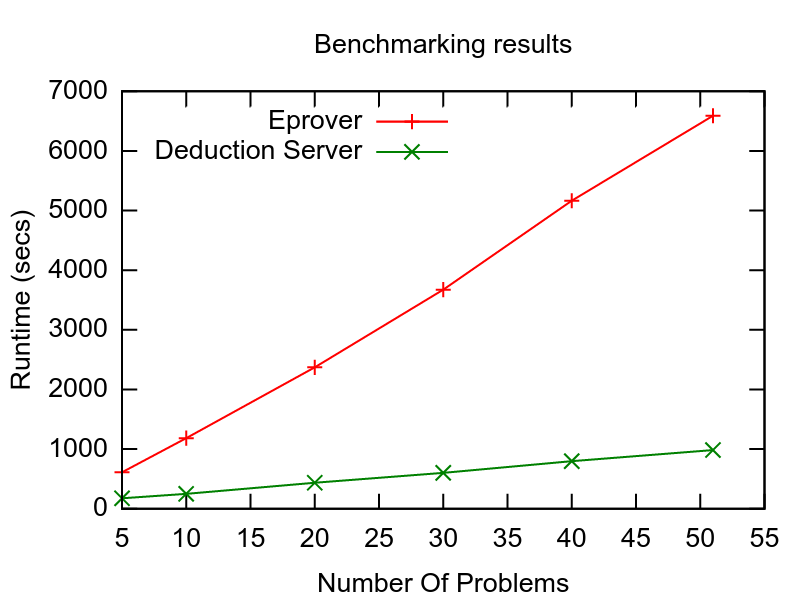
\includegraphics[width=0.75\textwidth]{imgs/BenchmarkingResults.png}
  \caption{Benchmarking Results\label{benchmarking_results}}
\end{figure}

The results in Figure~\ref{benchmarking_results} show the difference
between the single strategy server mode and the conventional
prover. The figure shows the accumulated wall-clock time over the
number of problems for which a proof was attempted.  In the
conventional case, the prover has to parse and index the axiom set for
each proof attempt. In the deduction server, the axioms are parsed and
indexed for axiom selection only once. The are then kept in the
server's memory and multiple queries can be executed against this
axiom set. Thus, the pre-processing time of each problem in the single
strategy server mode is amortized over multiple runs.

\section{Conclusion}
\label{sec:conc}

We have described the first implementation of a Deduction Server and
have introduced a communication protocol that supports remote
reasoning over largely fixed but flexible domains as a service. Our
results shows that the deduction server, even if configured for
identical pruning and search strategies, improves the run time for sets
of related problems by a significant amount, due to the amortization
of costs for parsing and the indexing needed for axiom
selection. This clearly shows that the approach is feasible and has
promise even if looking at it only from a performance point of view.

In addition to these performance benefits, having a formal protocol to
communicate with the prover over the net makes integrating it with
other applications much easier. Having access to a remotely running
prover is a win for those who can't install provers locally, e.g. for
OS compatibility issues or due to insufficient local computing
resources.

Future work includes improved multi-user support, in particular
controlling both access, but also the resources, such as CPU time and
memory, allocated for each user. Another important step would be the
integration of multiple deduction systems in the back-end, to improve
overall performance. This would offer a single interface to
potentially very diverse deduction systems. 

Finally, the Deduction Server can be extended to a cluster of servers,
to offer real scalable deduction as a service. In the simplest
version, a single head node accepts and processes user commands,
pre-processes the problems, and distributes the deduction jobs to
different servers. An even more scalable version would maintain
different user sessions with the current axiomatization on dedicated
machines, so that axiom selection can also be distributed.


%\bibliography{stsbib}

\begin{thebibliography}{10}

\bibitem{BN:IJCAR-2010}
Sascha B{\"o}hme and Tobias Nipkow.
\newblock {Sledgehammer: Judgement Day}.
\newblock In J{\"u}rgen Giesel and Reiner H{\"a}hnle, editors, {\em Proc.\ of
  the 5th IJCAR, Edinburgh}, volume 6173 of {\em LNAI}, pages 107--121.
  Springer, 2010.

\bibitem{GK:CPP-2015}
Thibault Gauthier and Cezary Kaliszyk.
\newblock {Premise Selection and External Provers for HOL4}.
\newblock In {\em Proceedings of the 2015 Conference on Certified Programs and
  Proofs}, pages 49--57, New York, NY, USA, 2015. ACM.

\bibitem{HHMNOZ:Kepler-2011}
Thomas~C. Hales, John Harrison, Sean McLaughlin, Tobias Nipkow, Steven Obua,
  and Roland Zumkeller.
\newblock A revision of the proof of the {K}epler conjecture.
\newblock In Jeffrey~C. Lagarias, editor, {\em The {K}epler Conjecture}, pages
  341--376. Springer, 2011.

\bibitem{HV:CADE-2011}
Kry\v{s}tof Hoder and Andrei Voronkov.
\newblock {Sine Qua Non for Large Theory Reasoning}.
\newblock In Nikolaj Bj{\o}rner and Viorica Sofronie-Stokkermans, editors, {\em
  Proc.\ of the 23rd CADE, Wroclav}, volume 6803 of {\em LNAI}, pages 299--314.
  Springer, 2011.

\bibitem{KU:JAR-2014}
Cezary Kaliszyk and Josef Urban.
\newblock Learning-assisted automated reasoning with {Flyspeck}.
\newblock {\em Journal of Automated Reasoning}, 53(2):173--213, 2014.

\bibitem{KE:SOSP-2009}
Gerwin Klein, Kevin Elphinstone, Gernot Heiser, June Andronick, David Cock,
  Philip Derrin, Dhammika Elkaduwe, Kai Engelhardt, Rafal Kolanski, Michael
  Norrish, Thomas Sewell, Harvey Tuch, and Simon Winwood.
\newblock {seL4}: Formal verification of an {OS} kernel.
\newblock In {\em Proc.\ of the 22nd ACM Symposium on Principles of Operating
  Systems (SOSPS)}, Big Sky, Montana, USA, October 2009. ACM.

\bibitem{KLTUH:CADE-2012}
Daniel K{\"u}hlwein, Twan van Laarhoven, Evgeni Tsivtsivadze, Josef Urban, and
  Tom Heskes.
\newblock Overview and evaluation of premise selection techniques for large
  theory mathematics.
\newblock In Bernhard Gramlich, Ulrike Sattler, and Dale Miller, editors, {\em
  Proc.\ of the 6th IJCAR, Manchester}, volume 7364 of {\em LNAI}, pages
  378--392. Springer, 2012.

\bibitem{McCune:JAR-1997}
William McCune.
\newblock {Solution of the Robbins problem}.
\newblock {\em Journal of Automated Reasoning}, 19(3):263--276, 1997.

\bibitem{McCune:Wos-1997}
W.W. McCune.
\newblock {33 Basic Test Problems: A Practical Evaluation of Some
  Paramodulation Strategies}.
\newblock In R.~Veroff, editor, {\em Automated Reasoning and its Applications:
  Essays in Honor of Larry Wos}, chapter~5, pages 71--114. MIT Press, 1997.

\bibitem{MP:JAR-2009}
Jia Meng and Lawrence~C. Paulson.
\newblock Translating higher-order clauses to first-order clauses.
\newblock {\em Journal of Automated Reasoning}, 40(1):35--60, 2008.

\bibitem{MP:JAL-2007}
Jia Meng and Lawrence~C. Paulson.
\newblock Lightweight relevance filtering for machine-generated resolution
  problems.
\newblock {\em Journal of Applied Logics}, 7(1):41--57, 2009.

\bibitem{PNL:AAAIWS-2002}
Adam Pease, Ian Niles, and John Li.
\newblock {The Suggested Upper Merged Ontology: A Large Ontology for the
  Semantic Web and its Applications}.
\newblock In {\em Working Notes of the AAAI-2002 Workshop on Ontologies and the
  Semantic Web}, 2002.

\bibitem{PS:IJCAR-2014}
Adam Pease and Stephan Schulz.
\newblock {Knowledge Engineering for Large Ontologies with Sigma KEE 3.0}.
\newblock In Stephane Demri, Deepak Kapur, and Christoph Weidenbach, editors,
  {\em Proc.\ of the 7th IJCAR, Vienna}, volume 8562 of {\em LNAI}, pages
  519--525. Springer, 2014.

\bibitem{RRG:CO-2005}
Deepak Ramachandran, Pace Reagan, and Keith Goolsbey.
\newblock {First-orderized ResearchCyc: Expressiveness and Efficiency in a
  Common Sense Knowledge Base}.
\newblock In Pavel Shvaiko, editor, {\em Proc.\ of the AAAI Workshop on
  Contexts and Ontologies: Theory, Practice and Applications (C\&O-2005)},
  2005.

\bibitem{Schulz:AICOM-2002}
S.~Schulz.
\newblock {E -- A Brainiac Theorem Prover}.
\newblock {\em Journal of AI Communications}, 15(2/3):111--126, 2002.

\bibitem{Schulz:LPAR-2013}
Stephan Schulz.
\newblock {System Description: E~1.8}.
\newblock In Ken McMillan, Aart Middeldorp, and Andrei Voronkov, editors, {\em
  Proc.\ of the 19th LPAR, Stellenbosch}, volume 8312 of {\em LNCS}. Springer,
  2013.

\bibitem{Sutcliffe:JAR-2009}
Geoff Sutcliffe.
\newblock {The TPTP Problem Library and Associated Infrastructure: The FOF and
  CNF Parts, v3.5.0}.
\newblock {\em Journal of Automated Reasoning}, 43(4):337--362, 2009.

\bibitem{Sutcliffe:LPAR-2010}
Geoff Sutcliffe.
\newblock The {TPTP World} - infrastructure for automated reasoning.
\newblock In E.~Clarke and A.~Voronkov, editors, {\em {Proc.\ of the 16th LPAR,
  Dakar}}, number 6355 in LNAI, pages 1--12. Springer, 2010.

\bibitem{SSSU:TPTP-ANS}
Geoff Sutcliffe, Mark Stickel, Stephan Schulz, and Josef Urban.
\newblock {Answer Extraction for TPTP}.
\newblock
  \url{http://www.cs.miami.edu/~tptp/TPTP/Proposals/AnswerExtraction.html}.
\newblock (acccessed 2013-07-08).

\bibitem{TB:IJCAI-1985}
Andrzej Trybulec and Howard~A. Blair.
\newblock Computer assisted reasoning with {MIZAR}.
\newblock In {\em Proc.\ of the 9th IJCAI, Los Angeles}, volume~85, pages
  26--28. Morgan Kaufmann, 1985.

\end{thebibliography}


\end{document}

%%% Local Variables: 
%%% mode: latex
%%% eval: (tex-pdf-mode)
%%% TeX-master: t
%%% End: 
